\begin{figure}[bth!]
  \begin{center}
	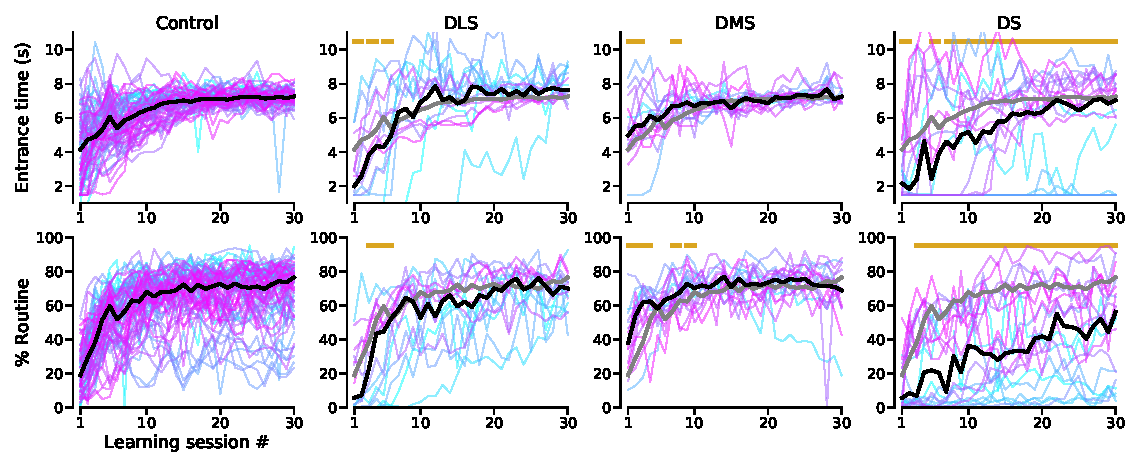
\includegraphics[scale=1]{ch-lesion/figures/EarlyLesionLearning.pdf}
	\caption[Effects of Striatal Lesions on Learning]
	{\textbf{Effect of DLS, DMS and DS lesions performed before training on task learning.}
	Session-by-session change in performance (ET, upper panels; Percentage of trials in which the routine was used, lower panels) for animals without lesion (Control, left) and for animals that received a lesion before training (DLS, DMS, DS from left to right). 
	Thick black lines show indicate group average.
    Thin colorful lines indicate single animals.
    Thick gray lines in 3 rightmost columns indicate control performance for comparison.
    Horizontal golden lines indicate significant differences between control and lesion groups. 
	}
	\label{fig:lesion:EarlyLesionLearning}
  \end{center}
\end{figure}